\documentclass[a4paper,11pt]{article}

\usepackage[english,brazil]{babel}
\usepackage[utf8]{inputenc}
\usepackage{amsmath}
\usepackage{algorithm}
\usepackage{algpseudocode}
\usepackage{graphicx}
\usepackage{fancyhdr}
\usepackage{url}
\renewcommand{\baselinestretch}{1.5}
\usepackage{titling}
\usepackage{geometry}
\usepackage{indentfirst}
\geometry{
	a4paper,
	left=25mm,
	right=25mm,
	top=1in,
	bottom=1in,
}
\usepackage{amsmath}
\usepackage{amssymb}
\usepackage{subfig}
\usepackage{multirow}
\usepackage[table]{xcolor}
\usepackage[backend=bibtex,style=ieee,sorting=none]{biblatex}
\bibliography{bibliography.bib}

\newcolumntype{C}{>{\centering\arraybackslash}p{1em}}

\title{\textbf{Controle de motor elétrico Brushless para robô jogador de futebol Small Size}}

\author{Aloysio Galvão Lopes, Prof. Dr. Carlos César Aparecido Eguti\\
	Instituto Tecnológico de Aeronáutica\\
	São José dos Campos, SP, Brasil} %\\

\date{\today}

% ADD THE FOLLOWING COUPLE LINES INTO YOUR PREAMBLE
\let\OLDthebibliography\thebibliography
\renewcommand\thebibliography[1]{
	\OLDthebibliography{#1}
	\setlength{\parskip}{0pt}
	\setlength{\itemsep}{0pt plus 0.3ex}
}


% O DOCUMENTO COME�A AQUI
\begin{document}
	
	\tableofcontents
	\newpage

	\maketitle
	
	\section{Plano Inicial}
	\textbf{1º bimestre (ago/set)} %Conferir
	\begin{itemize}
		\item Estudar controle de formal geral e estudar os mecanismos de controle de motores Brushless.
	\end{itemize}
	\textbf{2º bimestre (out/nov)}
	\begin{itemize}
		\item Estabelecer o sistema físico e projetar o mecanismo eletrônico para controle do motor.
		\item  Realizar simulação de tal mecanismo.
	\end{itemize}
	\textbf{3º bimestre (dez/jan)}
	\begin{itemize}
		\item Estabelecer método de testes eficiente e confeccionar o mecanismo de controle do motor.
		\item Confecção do relatório parcial.
	\end{itemize}
	\textbf{4º bimestre (fev/mar)} %Conferir
	\begin{itemize}
		\item Realizar testes iniciais e buscar otimizações no sistema de controle confeccionado.
	\end{itemize}
	\textbf{5º bimestre (abr/mai)}
	\begin{itemize}
		\item Projetar um novo sistema eletrônico compatível com as características do protótipo do robô Small Size da ITAndroids.
	\end{itemize}
	\textbf{6º bimestre (jun/jul)}
	\begin{itemize}
		\item Implementar o sistema de controle no protótipo do Small Size da ITAndroids.
		\item Corrigir erros e buscar otimizações.
		\item Confecção do relatório parcial.
	\end{itemize}

	\section{Atividades realizadas}
	\textbf{(ago/set/out/nov/dez/jan)}
	\begin{itemize}
		\item Bolsa ainda não implementada
	\end{itemize}
	\textbf{(fev/mar)}
	\begin{itemize}
		\item Início das atividades e replanejamento devido à redução do tempo de vigência da bolsa.
		\item Realização do curso de controle aplicado fornecido pelo grupo de robótica ITAndroids.
		\item Estudo dos métodos de acionamento dos motores Brushless e do funcionamento mecênico dos motores BLDC o dos motores de passo.
	\end{itemize}
		\textbf{(abr/mai)}
	\begin{itemize}
		\item Continuidade do curso de controle e estudo do acionamento dos motores BLDC por meio de encoders e sensores de efeito Hall e estudo de técnicas para a montagem da tabela de comutação de um motor BLDC.
		\item Realização do projeto e montagem do hardware para o primeiro teste de rotação do um motor (com BLDC retirado de drive de CD) em loop aberto e realização do teste de rotação.
		\item Estudo da modelagem física de motores elétricos DC e compreensão das diferenças da modelagem de um motor BLDC.
	\end{itemize}
		\textbf{(jun/jul)}
		\begin{itemize}
			\item Adaptação do hardware para o teste de controle do motor Maxon 45fl-200142, utilizado no robô Small Size e realização de seu controle com o auxílio dos sensores de efeito hall, bem como integração inicial à estrutura mecânica do robô.
			\item Modelagem do motor, desenvolvimento de um controlador PI e posterior simulação por meio do software MATLAB \cite{MATLAB}.
			\item Implementação do controlador PI em C++ para teste no motor e coleta dos resultados finais do projeto.
			\item Confecção do relatório final.
		\end{itemize}
	\section{Descrição do Problema}
		A ITAndroids, equipe de robótica do ITA, é uma iniciativa de alunos do ITA que representa a instituição em diversas competições de robótica nacionais e internacionais. O principal objetivo dessa iniciativa é a integração dos alunos com atividades de pesquisa em engenharia, em especial em robótica e inteligência artificial.
		
		A ITAndroids acredita que o hardware é fundamental no desenvolvimento de qualquer projeto de robótica, por isso, recentemente tem-se investido bastante no desenvolvimento dessa área. O desenvolvimento de conhecimento na área de controle de motores elétricos, assim, torna-se fundamental para a melhoria técnica da iniciativa.
		
		Nesse sentido, abre-se caminho para a participação na categoria Small Size, a qual necessita de uma eletrônica mais desenvolvida o que implica diretamente o desenvolvimento de conhecimento sobre controle de motores. Os motores utilizados para a locomoção dos robôs são motores Brushless, essa escolha se justifica pelo fato de que motores Brushless são mais eficientes, ocupam menos espaço e apresentam desgaste muito menor que motores DC tradicionais.
		
		Uma vez que o desgaste mecânico durante as partidas de futebol de robôs Small Size é elevado e é preciso alto rendimento dos sistemas mecânicos os motores BLDC são a escolha ideal; além disso, as principais equipes internacionais, tal como a equipe tailandesa SKUBA \cite{skuba} fazem uso de desses motores. Em contrapartida, o controle deste tipo de atuador mecânico se dá de maneira mais complexa uma vez que a comutação do campo magnético não é feita mecanicamente por escovas. A figura \ref{fig:esquemamotor}, abaixo, ilustra a mecânica de um motor BLDC.
		
		\begin{figure}[ht]
			\centering
			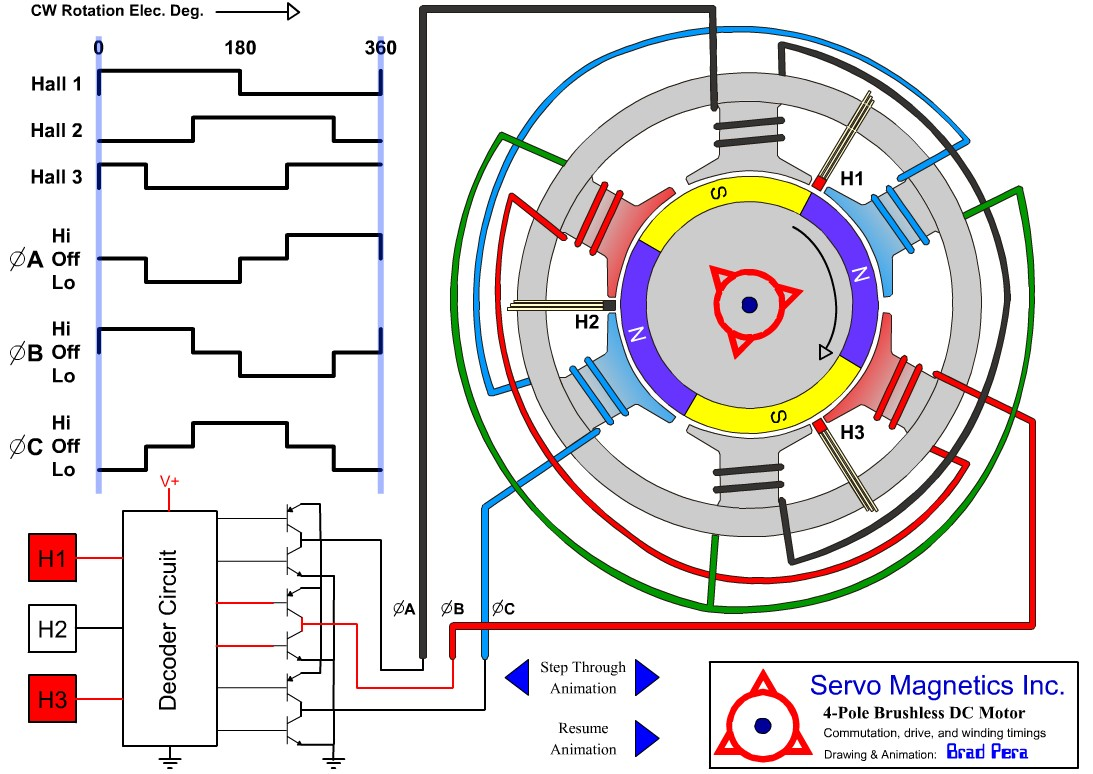
\includegraphics[width=0.7\linewidth]{images/4-Pole-brushless-DC-motor-animation}
			\caption{Esquema de um motor elétrico Brushless.}
			\label{fig:esquemamotor}
		\end{figure}
		
		
		O controle da comutação do campo magnético para esse tipo de motor é feito eletronicamente, o que acarreta a necessidade de um dispositivo eletrônico tal como um microcontrolador \cite{introducaobldc}. Isso aumenta a complexidade do sistema de locomoção como um todo, no entanto traz diversos ganhos em eficiência para o projeto.
		
		Nesse sentido o objetivo principal deste trabalho é compreender o funcionamento de um motor elétrico Brushless e ser capaz de realizar a comutação eletronicamente. Adicionalmente, deseja-se modelar o motor, simular e implementar um controlador PI para um motor Maxon 45fl-200142, o qual é utilizado para a locomoção de um robô Small Size.
	
	\section{Resultados}
		\subsection{Funcionamento de um motor elétrico Brushless}
		
		Um motor elétrico Brushless têm várias possíveis configurações, no entanto, a configuração trifásica ganha destaque. Isso pode ser constatado pela grande fabricação desse tipo de motor BLDC.
		
		Neste trabalho de iniciação científica é desenvolvido o controle de um motor da fabricante Maxon trifásico. Isso significa que existem três fases diferentes que devem ser eletronicamente comutadas para que se obtenha a rotação do motor. Além disso, o ciclo de rotação do motor é composto de seis etapas distintas, portanto o motor rotaciona com uma comutação de seis passos. Há apenas uma sequência correta de seis combinações das fases do motor para cada sentido de rotação.
		
		Vale destacar, também, que cada fase corresponde a uma bobina do motor e que estas bobinas estão interligadas. Assim, cada passo corresponde a aplicar tensão entre dois terminais de duas bobinas. As bobinas podem estar distribuídas ao redor da carcaça do motor, o que faz que uma rotação mecânica completa não seja equivalente a um ciclo elétrico. No caso do motor estudado, são necessárias 48 comutações para que uma revolução completa seja atingida; isso, portanto, significa que a cada oito ciclos elétricos ocorre um ciclo mecânico no motor. A figura \ref{fig:comutacao} abaixo ilustra a comutação de fases em um motor BLDC.
		
		\begin{figure}[ht]
			\centering
			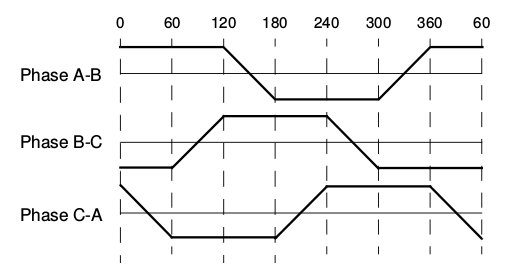
\includegraphics[width=0.7\linewidth]{images/comutacao}
			\caption{Três fases de um motor comutando \cite{introducaobldc}.}
			\label{fig:comutacao}
		\end{figure}
		
		
		Adicionalmente, é comum haver três sensores de efeito hall (é o caso deste motor), para que seja possível controlar a comutação. A combinação das três saídas de cada um dos sensores de efeito hall dá a próxima comutação a partir da tabela de comutação do motor.
		
		\subsection{Modelo utilizado no estudo}
		
		O modelo matemático utilizado no estudo do motor BLDC é o mesmo modelo utilizado para um motor DC convencional, o qual é uma boa aproximação para o modelo estudado \cite{modelomotor}. Considera-se que o torque produzido pelo motor é proporcional à corrente como mostrado em \ref{torquemotor} e que a tensão no motor é proporcional à velocidade angular $\dot{\theta}$, como mostrado em \ref{tensaomotor}.
		
		\begin{align}
			\tau = K_ti \label{torquemotor}\\
			V = K_b\dot{\theta} \label{tensaomotor}
		\end{align}
		
		Considerando, ainda, o momento de inércia do motor $J$ e que existe um atrito viscoso $b\dot{\theta}$, pela terceira lei de Newton, chega-se a \ref{leidenewtonmotor}. Utilizando a lei das malhas e considerando a queda de tensão devido à resistência do motor, à sua indutância e à conversão da energia em energia mecânica, sendo $\varepsilon$ a tensão da fonte, chega-se a \ref{malhasmotor}.
		
		\begin{align}
			J\ddot{\theta} = K_ti - b\dot{\theta} \label{leidenewtonmotor}\\
			\varepsilon = K_b\dot{\theta} + L\frac{di}{dt} + Ri \label{malhasmotor}
		\end{align}
		
		Pode-se, associando as equações \ref{leidenewtonmotor} e \ref{malhasmotor} chegar à função de transferência do motor, mostrada abaixo em \ref{plantamotor}. Observa-se que foram utilizados os dados fornecidos no pelo fabricante e foram desconsiderados os termos do atrito viscoso, pois eram negligenciáveis.
		
		\begin{equation}
			\frac{\dot{\Theta(s)}}{\varepsilon(s)} = \frac{13.095}{2.66 \cdot 10^{-6} s^2+0.0171s+1} \label{plantamotor}
		\end{equation}
		
		\subsection{Hardware confeccionado para acionamento do motor}
		
		Foi confeccionado um hardware para acionamento do motor baseado no esquema mostrado abaixo, na figura \ref{fig:diagrama}.
		
		\begin{figure}[ht]
			\centering
			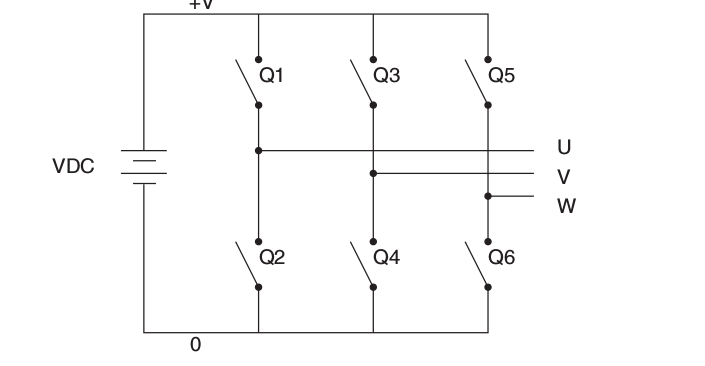
\includegraphics[width=0.7\linewidth]{images/circuitdiagram}
			\caption{Diagrama do circuito para acionamento do motor \cite{atmeldiagrama}.}
			\label{fig:diagrama}
		\end{figure}
	
		Foram utilizados seis pares darlington TIP 122 para montar o esquema mostrado acima de três meias pontes H e uma placa de desenvolvimento Arduino Mega ADK para o controle. O sistema inicialmente foi testado com um motor Brushless retirado de um drive de DVD em loop aberto. Observou-se que sem um feedback dos sensores a velocidade máxima atingida pelo motor era muito pequena e a rotação não se dava de maneira suave. Isso mostra que sem informações sobre a posição do rotor o rotor facilmente não é capaz de acompanhas a variação do campo magnético.
		
		Abaixo, é mostrada na figura \ref{fig:montagemcircuito} a montagem do circuito para o controle do motor. Na figura \ref{fig:motorantigo} é mostrado o motor de drive de DVD utilizado inicialmente.
		
		\begin{figure}[ht]
			\centering
			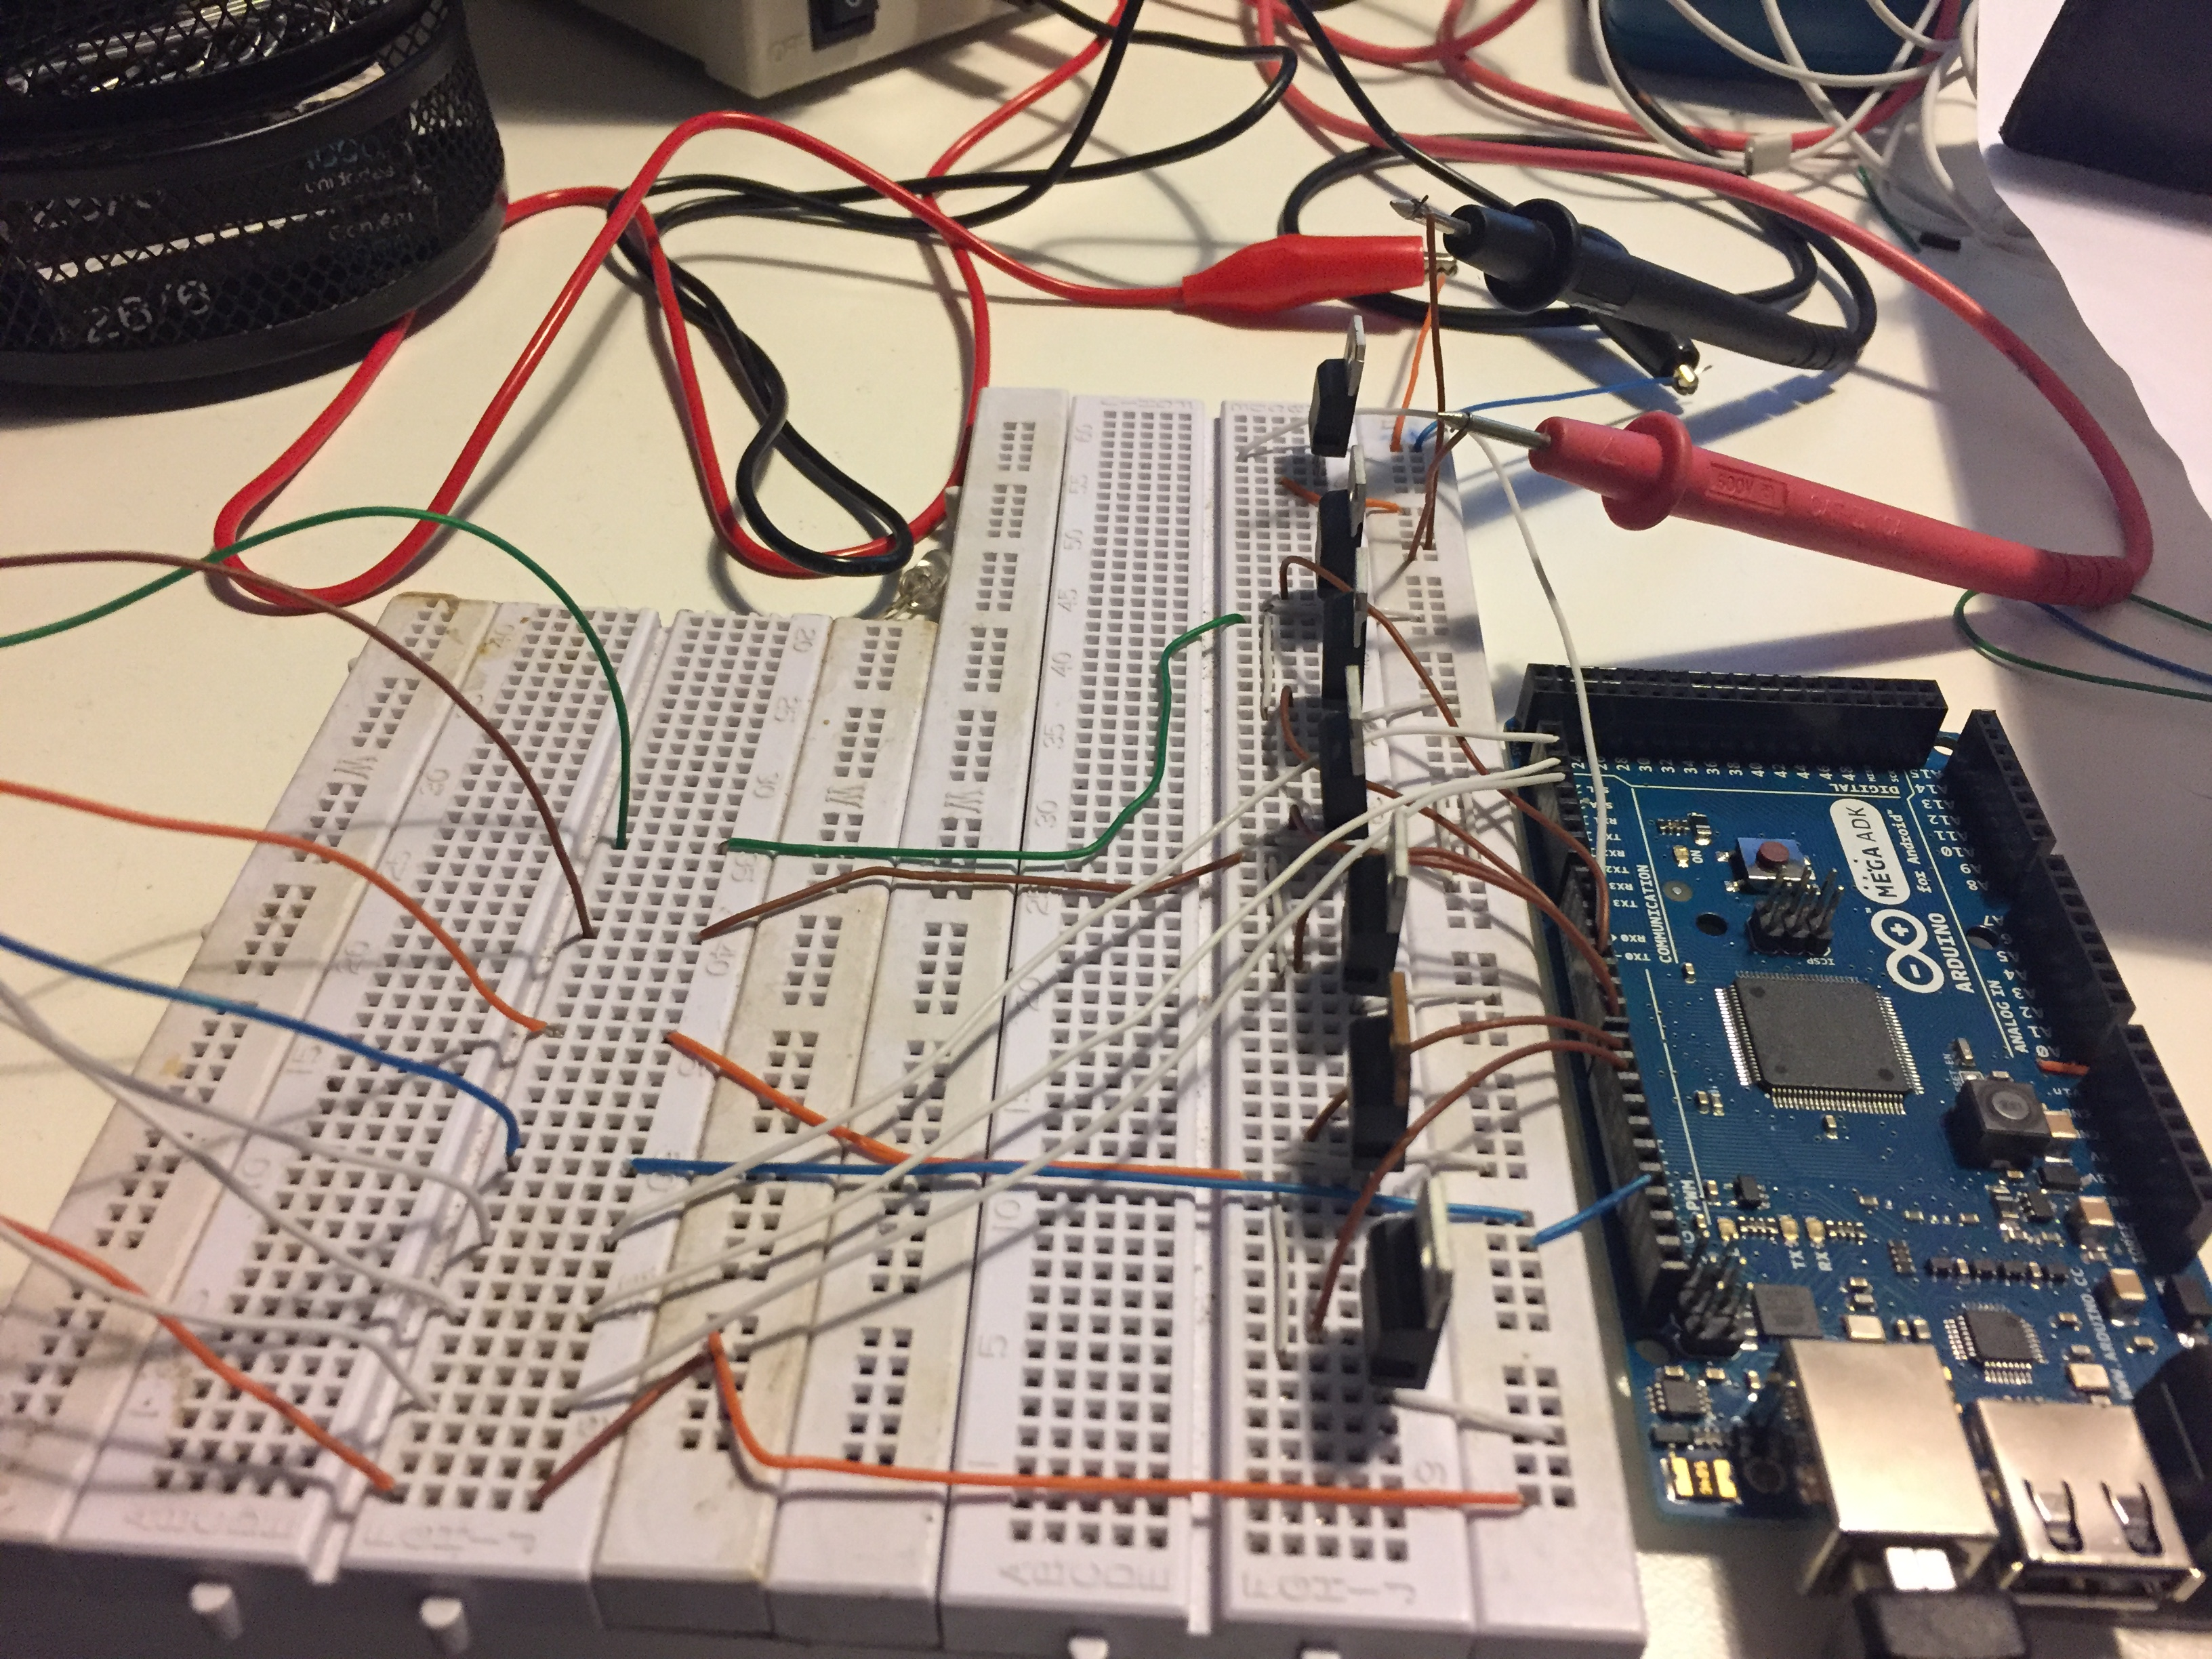
\includegraphics[width=0.5\linewidth]{images/montagemcircuito}
			\caption{Figura da montagem do circuito para controle do motor.}
			\label{fig:montagemcircuito}
		\end{figure}
		
		\begin{figure}[ht]
			\centering
			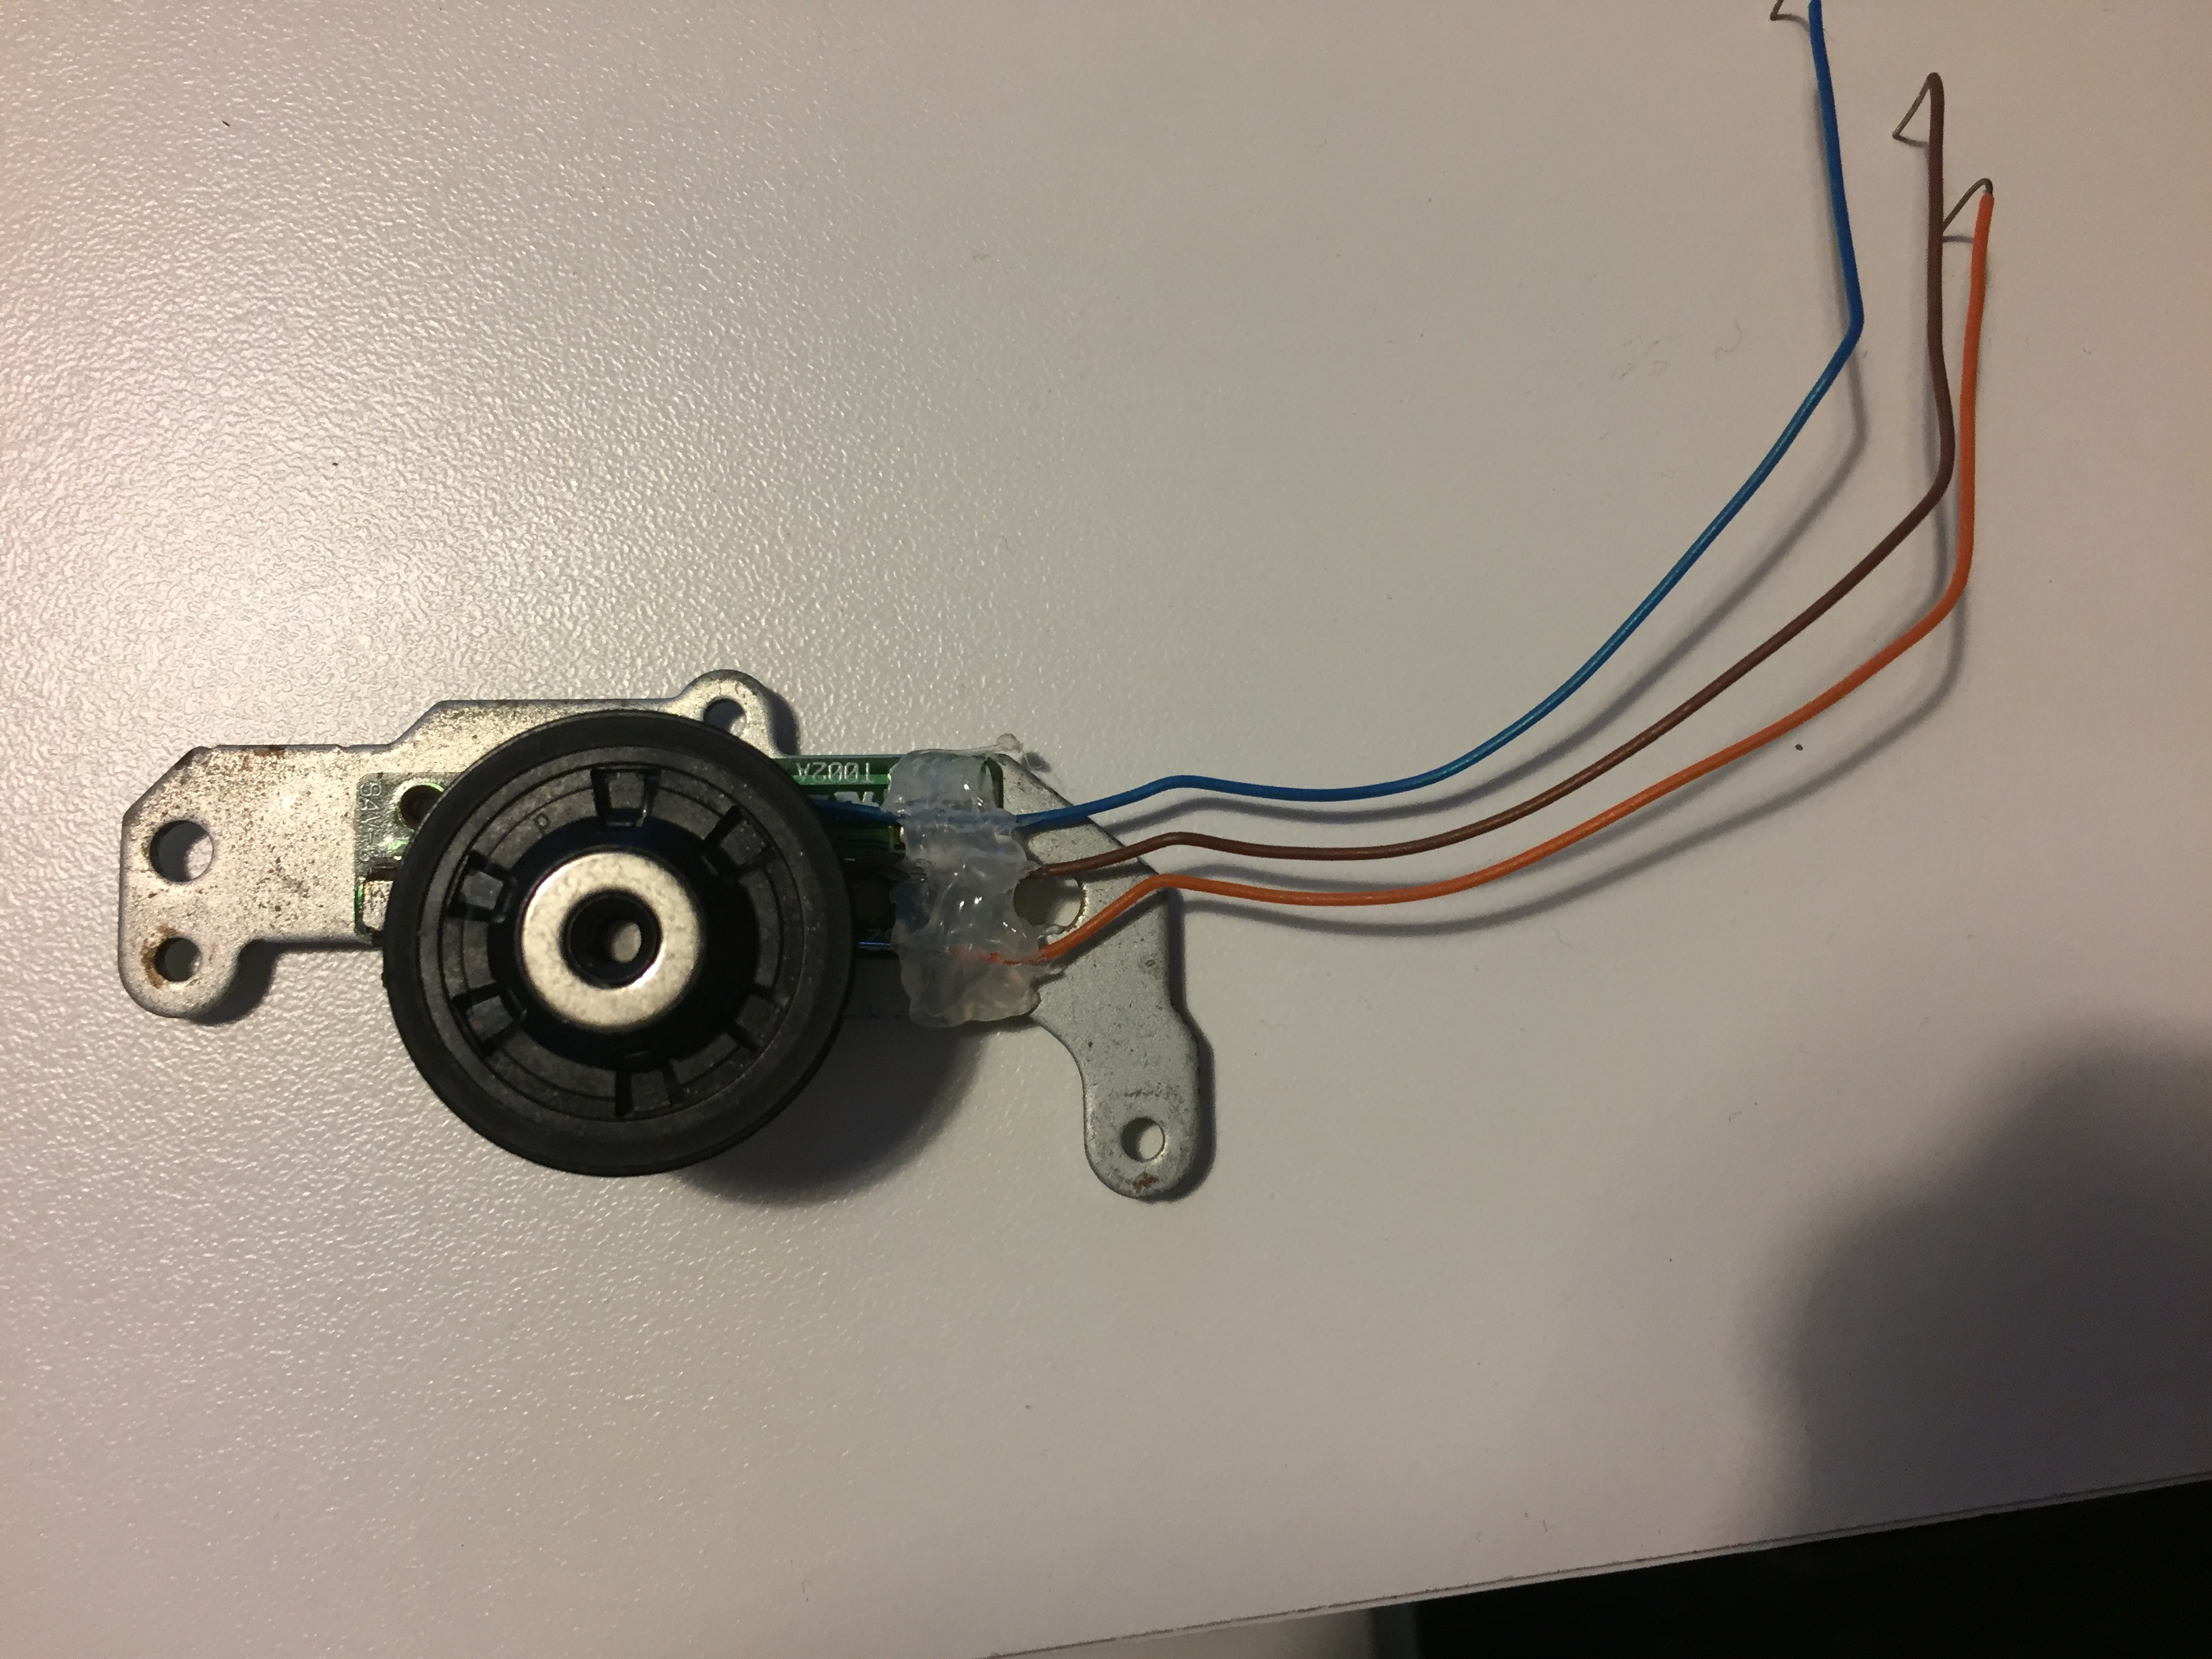
\includegraphics[width=0.5\linewidth]{images/motorantigo}
			\caption{Motor de drive de DVD utilizado nos teste, nota-se que não há saídas para sensores de efeito hall.}
			\label{fig:motorantigo}
		\end{figure}
	
		\newpage
		
		Em uma segunda etapa, utilizou-se o motor Maxon 45fl-200142, cujo controle é o objetivo deste estudo. Nesse caso, foi possível utilizar o feedback dos sensores de efeito hall e obter uma rotação suave, além disso, foi desenvolvido um script para a obtenção da tabela de comutação, uma vez que esta não é fornecida pelo fabricante. Este script pode ser posteriormente utilizado para a obtenção da tabela de comutação de qualquer motor Brushless. Vale ressaltar que a regulação da velocidade aqui é feita utilizando PWM. Para isso uma saída PWM é gerada para cada transístor que leva corrente do motor ao ground, seguindo o esquema mostrado em \ref{fig:esquemamotor}.
		A figura \ref{fig:motornovo}, abaixo, mostra o motor da Maxon rotacionando. Mais adiante serão tratados os aspectos de controle implementados.
		
		\begin{figure}[ht]
			\centering
			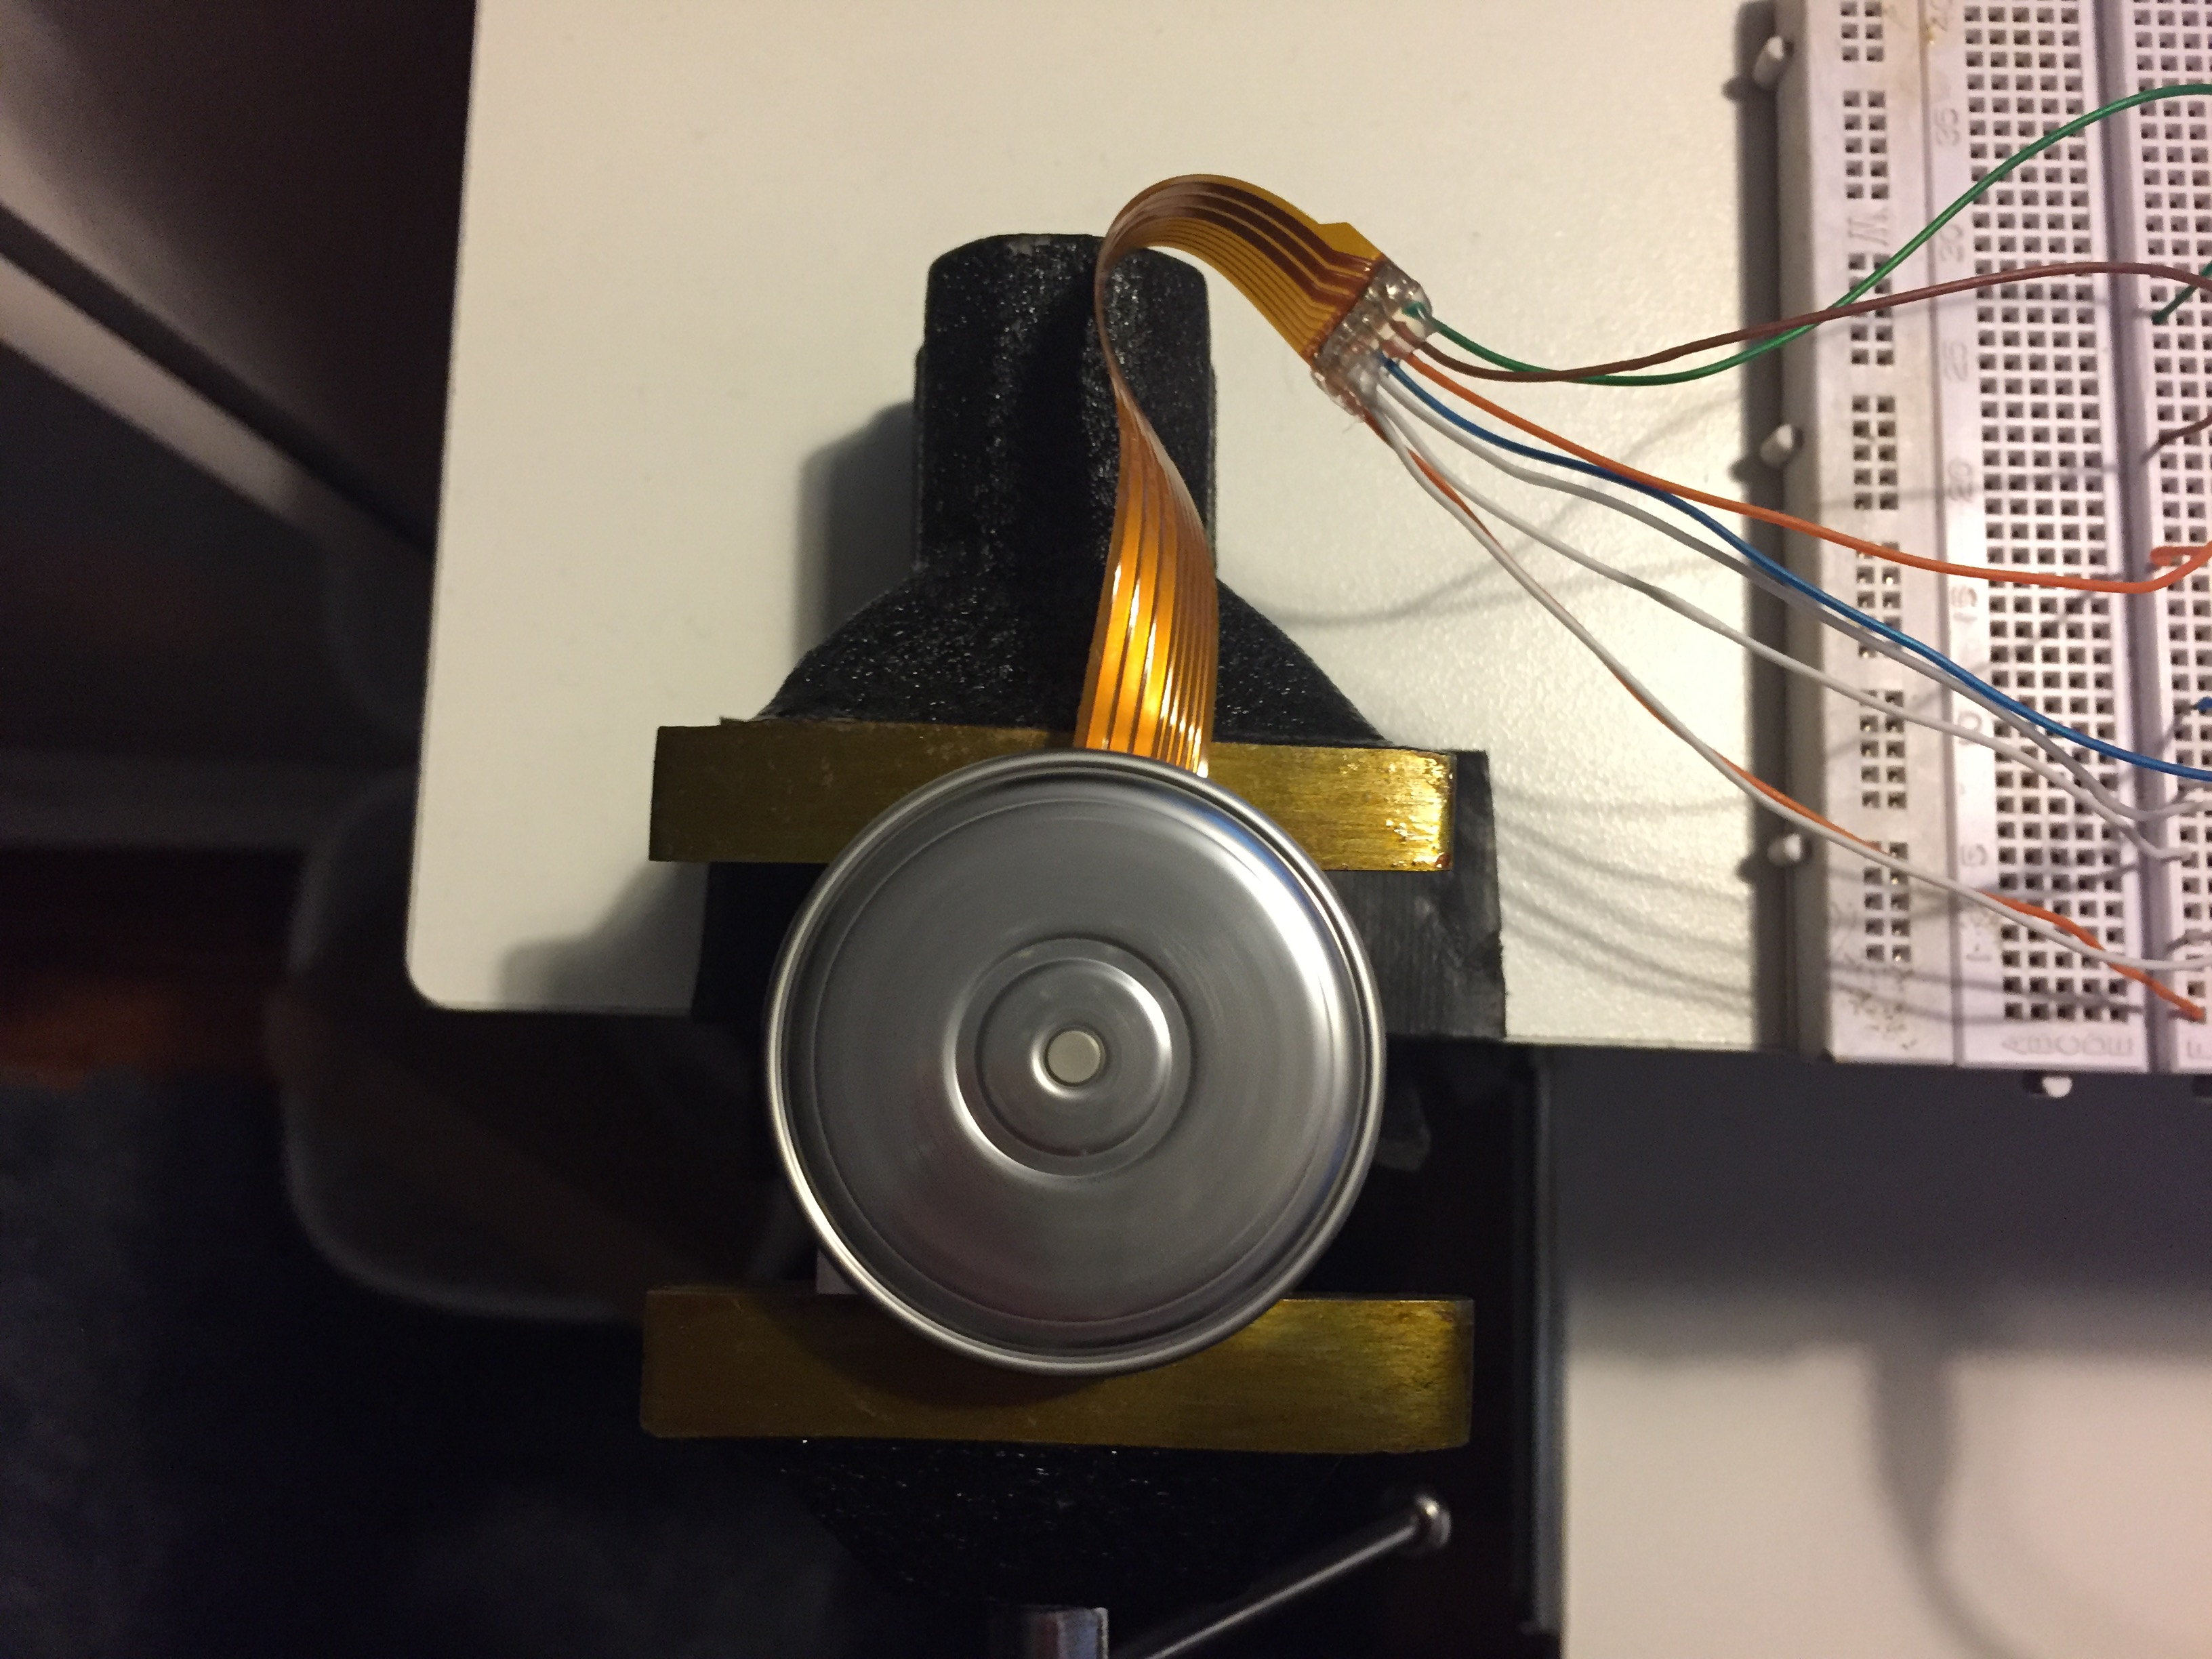
\includegraphics[width=0.5\linewidth]{images/motornovo}
			\caption{Motor Maxon 45fl-200142 rotacionando.}
			\label{fig:motornovo}
		\end{figure}
	
		\newpage
		
		\subsection{Simulação do modelo}
		
		Foi implementada em MATLAB\cite{MATLAB} a função de transferência \ref{plantamotor} e, com isso, foi possível obter os gráficos para a resposta em degrau do sistema, bem como o diagrama de Bode. As figuras \ref{respostaemdegrau} e \ref{bode}, respectivamente, representam a resposta em degrau unitário e o diagrama de Bode da planta obtidos.
		
		\subsection{Análise do resultados no motor Maxon 45fl-200142}
	\section{Conclusão}
	
	\section{Agradecimentos}
	Agradeço ao CNPQ, pelo apoio financeiro durante a realização do projeto, bem como ao meu professor orientador pelo apoio à realização do projeto. Agradeço à iniciativa ITAndroids, por fornecer os treinamentos necessários e recursos materiais para a realização do projeto.
	
	\section{Bibliografia}
	%\bibliographystyle{IEEEtran}
	%\bibliographystyle{bibstyle}
	\printbibliography[heading=none]
	
\end{document}